\section{Кинематика прямолинейного движения материальной точки}

\begin{ex} %ПодОл2-6
Координата движущейся по прямой точки меняется по закону: $x = 2 + 10t + 3t^2$ ($x$ измеряется в метрах, $t$ в секундах). Какова ее скорость при $t = 2$ с?
\begin{ans}
$v = 22$ м/с.
\end{ans}
\end{ex}

\begin{ex} %ПодОл2-7
Показать, что средняя скорость за промежуток времени от $t_1$ до $t_2$ при равноускоренном движении равна скорости в момент времени $(t_1 + t_2)/2$.
\begin{ans}
\end{ans}
\end{ex}

\begin{ex} %ПодОл2-9 
От движущегося поезда отцепляют последний вагон. Поезд продолжает движение с той же скоростью $v_0$. Как будут относиться пути, пройденные поездом и вагоном к моменту остановки вагона? Считать, что вагон движется равнозамедленно. Решить задачу аналитически и графически.
\begin{ans}
2.
\end{ans}
\end{ex}

\begin{ex} %ПодОл2-13
Машинист пассажирского поезда, двигавшегося со скоростью $v_1 = 108$ км/ч, заметил на расстоянии $S_0 = 180$ м впереди движущийся в ту же сторону со скоростью $v_2 = 32,4$ км/ч товарный поезд. Машинист сразу включил тормоз, благодаря чему пассажирский поезд начал двигаться с ускорением $a = -1,2$ м/с\textsuperscript{2}. Достаточно ли этого ускорения для того, чтобы поезда не столкнулись?
\begin{ans}
Нет.
\end{ans}
\end{ex}

\begin{ex} %Сив13
Тело, двигаясь с постоянным ускорением, проходит последовательно два одинаковых отрезка пути $S$ по 10 м каждый. Найти ускорение тела $a$ и скорость $v_0$ в начале первого отрезка, если первый отрезок пройден телом за время $t_1 = 1,06$ с, а второй за $t_2 = 2,2$ с.
\begin{ans}
$a = \frac{2S\left(t_1-t_2\right)}{t_1t_2\left(t_1+t_2\right)} \approx -3$ м/c\textsuperscript{2} , $v_0 = \frac{S}{t_1}-\frac{at_1}{2} \approx 11,5$ м/с.
\end{ans}
\end{ex}

\begin{ex} %Сив14
Начертить графики зависимости от времени скорости некоторых тел, если графики ускорения $a$ этих тел имеют вид, представленный на рис. \ref{kinemGraph} (начальная скорость тел во всех случаях равна нулю).
\begin{figure}
\centering
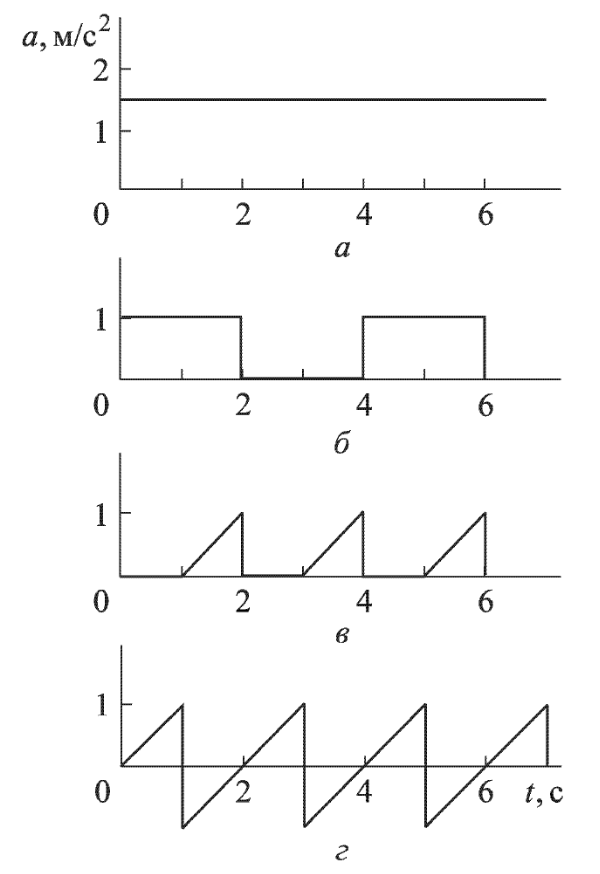
\includegraphics[width=0.5\textwidth]{kinemGraph.png}
\caption{}
\label{kinemGraph}
\end{figure}
\begin{ans}
\end{ans}
\end{ex}

\begin{ex} %ПодОл2-18
За последнюю секунду свободно падающее тело прошло $3/4$ всего пути. С какой высоты оно упало?
\begin{ans}
20 м.
\end{ans}
\end{ex}

\begin{ex} %Сив17
С вышки одновременно брошены два тела с одинаковой начальной скоростью $v_0$: одно вертикально вверх, другое вертикально вниз. Как с течением времени будет меняться расстояние $S$ между этими телами? Сопротивление воздуха движению тел не учитывать.
\begin{ans}
$S = 2 v_0 t$.
\end{ans}
\end{ex}

\begin{ex} %Сив33
Из точки, лежащей на верхнем конце вертикального диаметра некоторой окружности, по желобам, установленным вдоль различных хорд этой окружности, одновременно начинают скользить без трения грузы. Показать, что все грузы достигнут окружности одновременно.
\begin{ans}
$t = \sqrt{2D/g}$.
\end{ans}
\end{ex}

\begin{ex} %Сив15
Начертить графики зависимости от времени пути и ускорения некоторого тела, если скорость этого тела как функция времени представлена графиком на рис. \ref{kinemGraphAccel}.
\begin{figure}
\centering
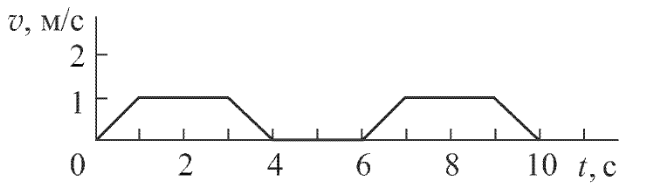
\includegraphics[width=0.7\textwidth]{kinemGraphAccel.png}
\caption{}
\label{kinemGraphAccel}
\end{figure}
\begin{ans}
\end{ans}
\end{ex}

\begin{ex} %ПодОл2-19
С каким ускорением движется тело, если за восьмую секунду после начала прямолинейного движения оно прошло путь 30 м.
\begin{ans}
4 м/с\textsuperscript{2}.
\end{ans}
\end{ex}

\begin{ex} %ПодОл2-34
Трамвай тормозит с постоянным ускорением до полной остановки. Найдите тормозной путь трамвая, если торможение заняло 5 с, а скорость трамвая на середине тормозного пути была 4 м/с.
\begin{ans}
$S = vt/\sqrt{2} = 14$ м.
\end{ans}
\end{ex}

\begin{ex} %ПодОл2-44
С высоты $H$ на упругую горизонтальную плиту свободно падает шарик. Построить график изменения координаты, скорость и ускорения шарика в зависимость от времени, считая, что временем соударения и сопротивлением воздуха можно пренебречь. Удар абсолютно упругий.
\begin{ans}
\end{ans}
\end{ex}

\begin{ex} %Чертов1.21
Тело, брошенное вертикально вверх, находилось на одной и той же высоте $h = 8,6$ м два раза с интервалом $\Delta t = 3$ с. Пренебрегая сопротивлением воздуха, вычислить начальную скорость брошенного тела.
\begin{ans}
19,6 м/c
\end{ans}
\end{ex}

\begin{ex} %Чертов1.22
С балкона бросили мячик вертикально вверх с начальной скоростью $v_0 = 5$ м/с. Через $t = 2$ с мячик упал на землю. Определить высоту балкона над землей и скорость мячика в момент удара о землю.
\begin{ans}
9,62 м; 14,6 м/c
\end{ans}
\end{ex}

\begin{ex} %ПодОл2-50
Муравей бежит от муравейника по прямой так, что его скорость обратно пропорциональна расстоянию до центра муравейника. В тот момент, когда муравей находится в точке $А$ на расстоянии 1 м от центра муравейника, его скорость равна 2 м/c. За какое время муравей добежит от точки А до точки $B$, которая находится на расстоянии 2 м от центра муравейника?
\begin{ans}
0,75 с.
\end{ans}
\end{ex}

\clearpage